\section{Current project status}

We will now assess the current status of the project, giving a more thorough overview of the job done.

\subsection{Legal framework analysis}

One of the first aspects to bear in mind when developing a technological project is the legal environment in which it is framed.

Concerning the actual code base of the project, we must implement all necessary intellectual property protection measures. Because it is an \textit{open source} project, an internationally recognised software license will be included in the public code repository, hosted at GitHub\footnote{The project is available at \url{https://github.com/necavit/moa-ppsm}.}. The chosen license is the \href{http://opensource.org/licenses/MIT}{MIT License}, which has proven to be easy to understand, relatively widespread and quite permissive.

Within the project, no personal data has yet been used to perform any benchmarking process nor to assess the quality of the developed methods - random data generators are being used instead. However, if such data was ever used, it is clear that is should be under the terms of the spanish LOPD law and that, therefore, protection and security measures should be taken accordingly. It is unclear, at the moment, that any sensitive data set might be used throughout this project; many benchmark data sets available are free from any kind of sensitive, personal data.

We have not detected any other kind of legal consequences or regulations bound to this project's development.

\subsection{Technology alternatives}

Before we started developing privacy preservation filters, a number of existing technologies was considered as possible solutions for the goals of the project.

As for the proposed SDC methods to be developed, there is a popular library which implements all of them: \texttt{sdcMicro}~\cite{sdcMicro}. The main problem is that this piece of software is written in R, whereas the MOA framework is written in Java. An evaluation was performed to decide whether to use this library or to develop the privacy filters ourselves, from scratch.

\begin{figure}[h]
	\centering
	\begin{minipage}[t]{.45\textwidth}
		\centering
		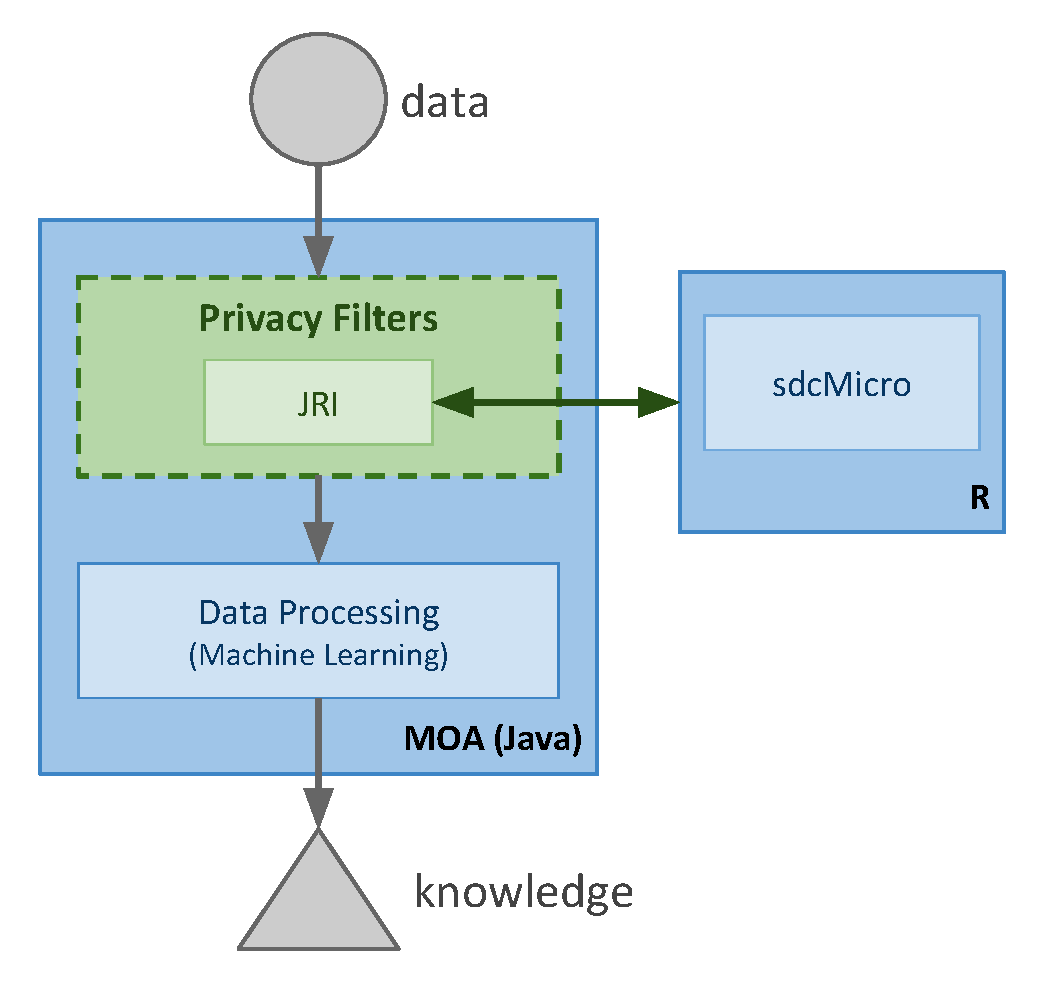
\includegraphics[width=1.0\textwidth]{figures/moa-ppsm-JRI.pdf}
		\caption{Data flow: R/Java hybrid solution.}
		\label{fig:ppsm-JRI}
	\end{minipage}\hfill
	\begin{minipage}[t]{.5\textwidth}
		\centering
		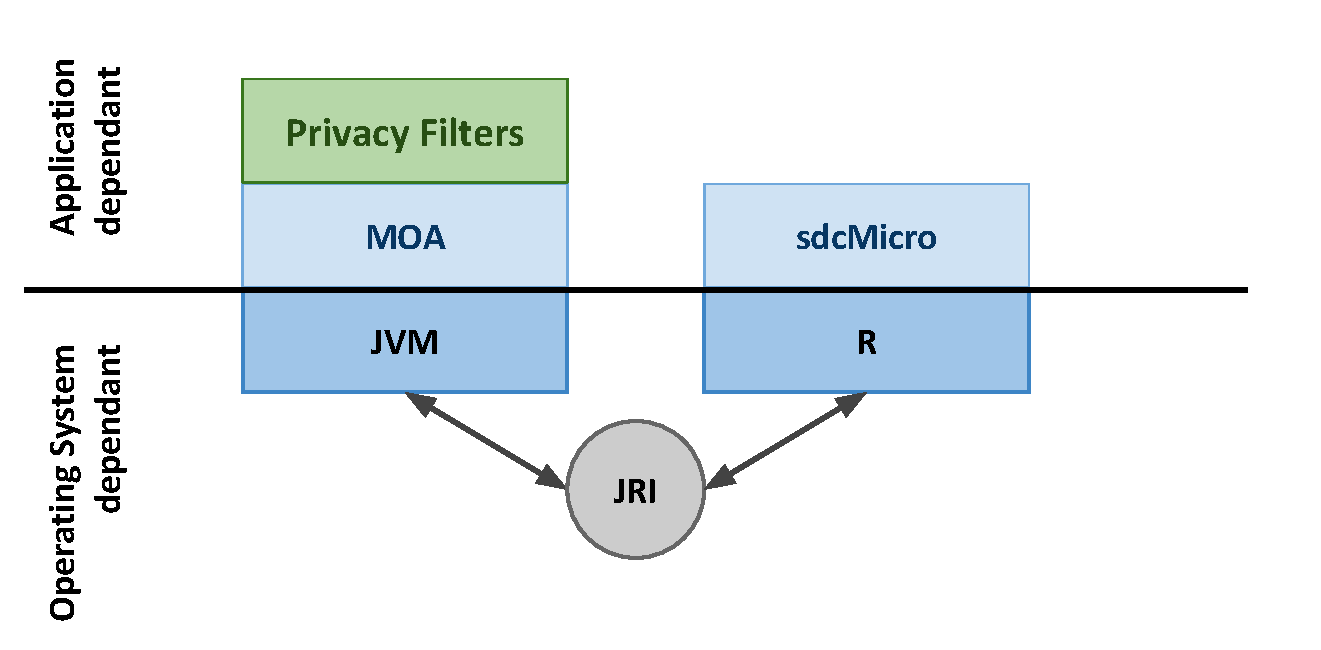
\includegraphics[width=1.2\textwidth]{figures/moa-ppsm-JRI-arch.pdf}
		\caption{Hybrid solution architechture: strong dependencies.}
		\label{fig:ppsm-JRI-arch}
	\end{minipage}
\end{figure}

As can be seen in figures \ref{fig:ppsm-JRI} and \ref{fig:ppsm-JRI-arch}, the \texttt{sdcMicro} library would be used from within MOA by using an adapter (a wrapper) to interconnect the Java and R execution environments. There are some benefits of taking this approach, but also some drawbacks, which are reflected in table~\ref{table:JRI-pros-cons}. This interconnection could be done using different technologies:

\begin{itemize}
	\item \textbf{rJava/JRI:} the \texttt{rJava} and \texttt{JRI} counterparts are a couple of libraries designed to provide low-level communication between the Java Virtual Machine (JVM) and an R process.
	\item \textbf{Rserve:} it is a TCP/IP server which allows other programs to use facilities of R from various languages without the need to initialize R or link against an R library.
\end{itemize}

Either solution implies that marshalling and unmarshalling techniques must be applied, in order to transform the data structures used by R and Java. Even though that no SDC algorithm would need to be implemented, the interconnect code would not be easy to maintain.

\begin{table}[h]
	\centering
	\begin{tabular}{ll}
		\hline
		\textbf{Benefits}     & \textbf{Drawbacks}                     \\ \hline
		Faster development    & No algorithms are indeed developed     \\
		Easily extensible     & Strong dependencies                    \\
		SDC methods are right & Depends on external installed software \\
		                      & Needs system libraries to work         \\
		                      & Maintanability is harder               \\
		                      & Reduced performance due to marshalling \\ \hline
	\end{tabular}
	\caption{Evaluation of the R/Java hybrid solution.}
	\label{table:JRI-pros-cons}
\end{table}

There is still another possibility that would allow using the \texttt{sdcMicro} library: the Renjin project~\cite{website:renjin}. Renjin is a JVM-based interpreter for the R language: all computations of any R package can be executed upon the JVM, instead of a separate R process. This way, the dependency that this project could have on R and some system libraries disappears. However, it is worth noting that, even with Renjin, data structures conversion would have to be performed, rendering its use as impractical as the use of JRI. Moreover, the \texttt{sdcMicro} package was still not available in its JVM port at the time of the evaluation due to some dependencies and errors, and we could not wait for it to be solved.

After considering the above alternatives, we decided to go for a pure native Java implementation of the proposed SDC methods. This way, portability and performance are increased, complexity is reduced (in terms of the necessary infrastructure), strong dependencies are avoided (no more system libraries must be installed) and last, but not least, the filters and developed methods can be adapted to a more streaming-prone processing style. Figures~\ref{fig:ppsm-JAVA} and~\ref{fig:ppsm-JAVA-arch} show how the system is built, in general terms.

\begin{figure}[h]
	\centering
	\begin{minipage}[t]{.45\textwidth}
		\centering
		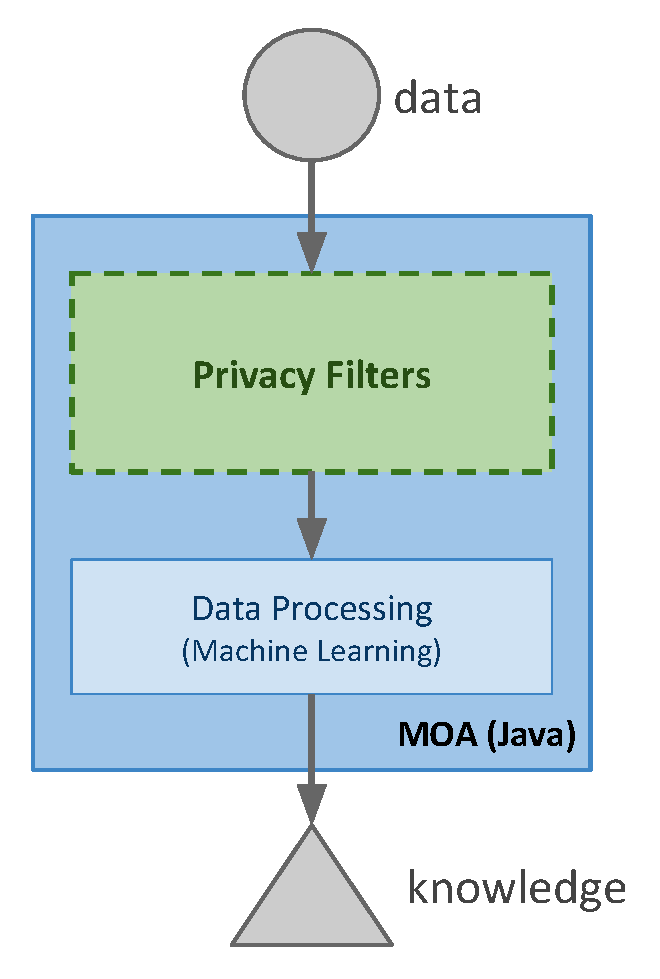
\includegraphics[width=.7\textwidth]{figures/moa-ppsm-JAVA.pdf}
		\caption{Data flow: pure Java solution.}
		\label{fig:ppsm-JAVA}
	\end{minipage}\hfill
	\begin{minipage}[t]{.45\textwidth}
		\centering
		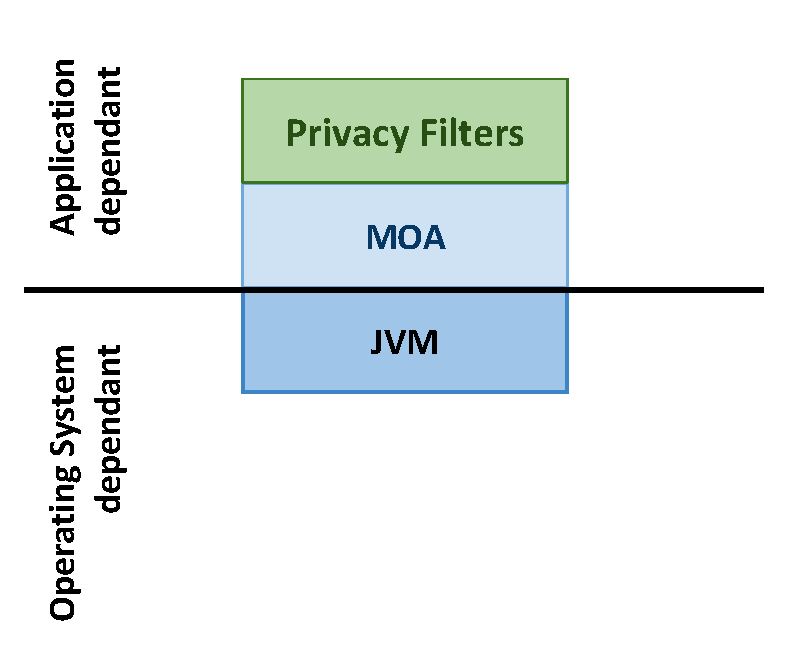
\includegraphics[width=1.0\textwidth]{figures/moa-ppsm-JAVA-arch.pdf}
		\caption{Pure Java solution architechture: few dependencies.}
		\label{fig:ppsm-JAVA-arch}
	\end{minipage}
\end{figure}

\subsection{Implemented algorithms}

Some of the privacy preserving algorithms proposed at the beginning of the project have been already developed (as was stated in section~\ref{section:project_management}).

As a quick note, the current microaggregation filter implementation uses a $k$-Nearest Neighbors approach for the clustering stage of the process, instead of some other more complex and costly solutions, like the MDAV algorithm. All other filters implemented are basic variants of the papers already cited in section~\ref{section:project_management}.

An incomplete UML class diagram of the current work is shown in figure~\ref{fig:ppsm-class-diagram}. It is perhaps confusing to separate anonymization algorithms from privacy filters, but this design solution aims to provide a \textit{framework} structure for the project, using the \textit{inversion of control} pattern, also known as the \textit{Hollywood principle}~\cite{website:wikiInversionOfControl}. The idea behind it is that \texttt{AnonymizationAlgorithm}s are completely independent of the conceptual \texttt{PrivacyFilter} wrappers that use them: filters like the \texttt{NoiseAdditionFilter} inject the necessary SDC algorithm on construction. Therefore, end users do not need to instantiate the algorithms and pass them to a generic filter themselves.

\begin{figure}[h]
	\centering
	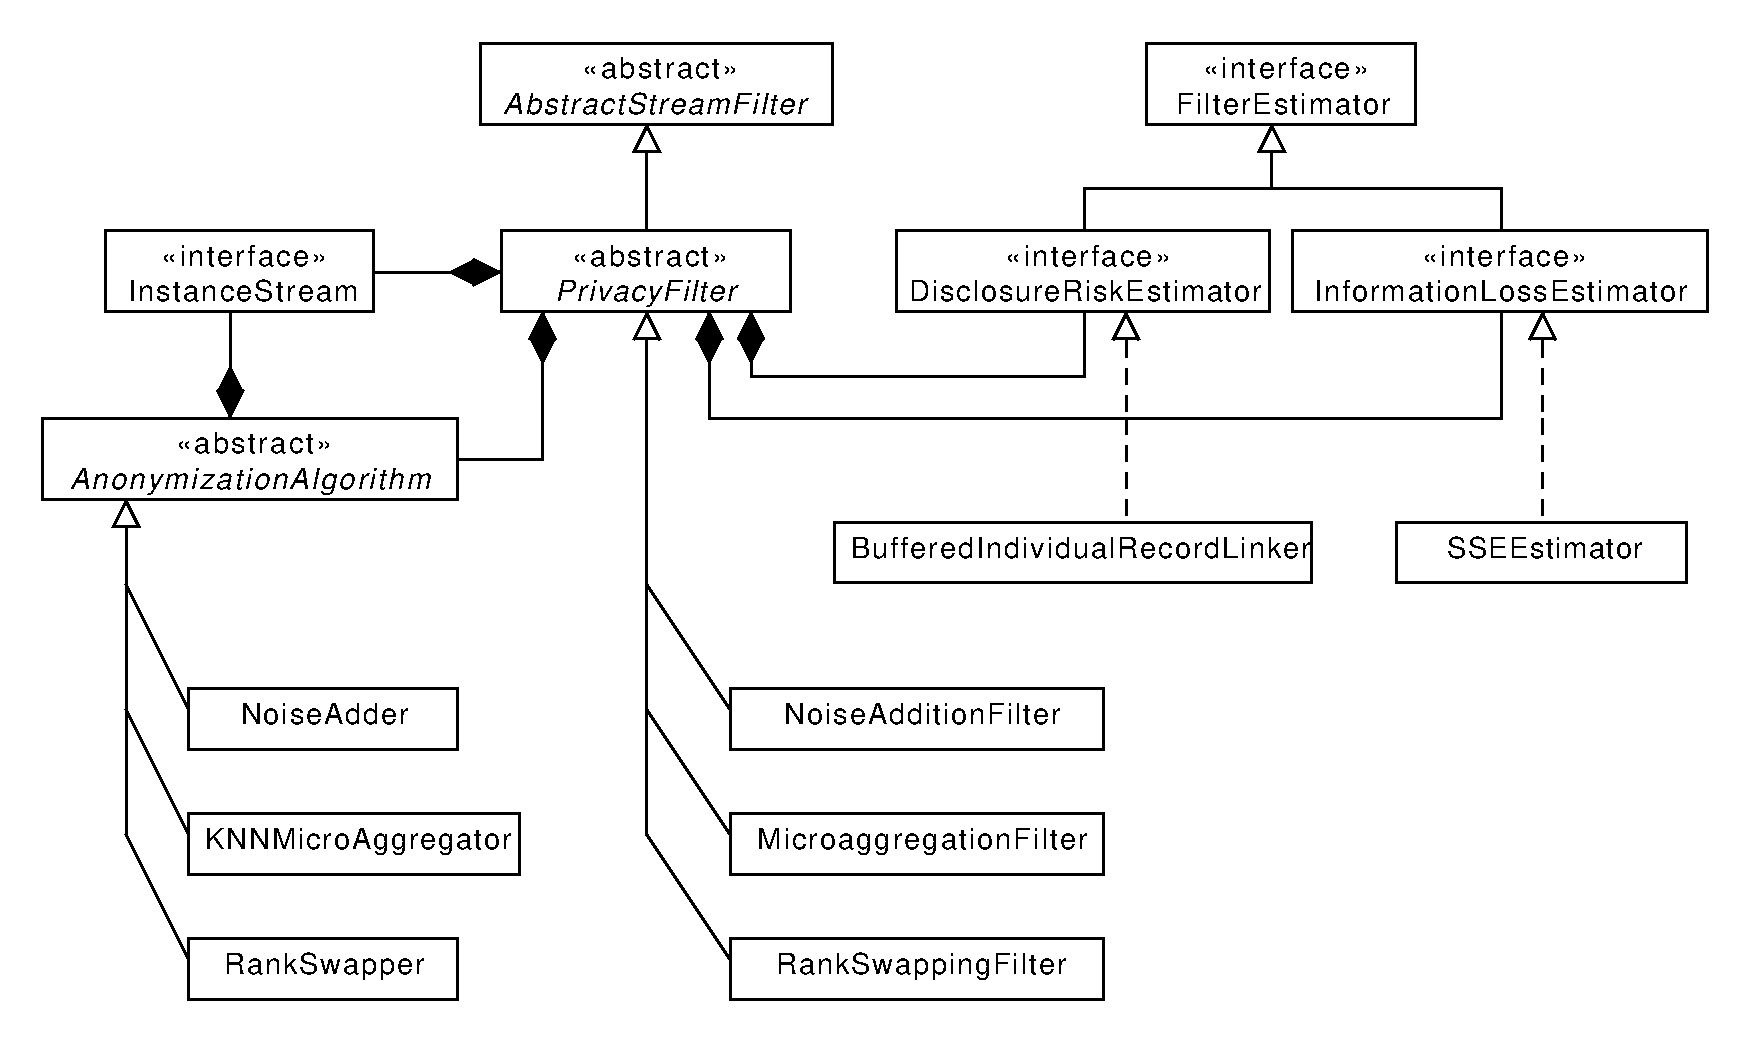
\includegraphics[width=1.0\textwidth]{figures/ppsm-class-diagram.pdf}
	\caption{Partial view of the \texttt{moa-ppsm} class diagram.}
	\label{fig:ppsm-class-diagram}
\end{figure}
